\hfill

\section{Quantum Prisoners' Dilemma}
In this section will be analyzed and simulated a canonical non-zero sum game usually known as the prisoners' dilemma. In these kind of games, in contrast to zero-sum games, the two players no longer appear in strict opposition to each other, but may rather benefit from mutual cooperation. \\
\textit{
Note. All the plots shown in this section have been realized in Python: the original code is contained in a Jupyter Notebook that can be found on Github \cite{Pujatti_github}. It may be useful to give a look there if interested in a computational implementation of this problem and/or a deeper overview of it.}\\
There are two players, Alice and Bob, that are thieves caught by the police, which are being questioned, and can choose among two strategies, Mum (collaborating, C) or Fink (defecting, D). The payoffs are distributed according table \ref{eq:pris_dilemma} and, as usually, the objective of each player is to maximize his or her individual utility.
\begin{equation}
\begin{blockarray}{cccc}
& & \text{Player B}&\\
& & C & D\\
\begin{block}{cc[cc]}
\text{Player A} & C & 3,3 &  0,5 \\
 & D & 5,0 & 1,1 \\
\end{block}
\end{blockarray}
\label{eq:pris_dilemma}
\end{equation}
Analyzing the problem using classical game theory, one can conclude that the best strategy to be played is found at the Nash Equilibrium, i.e. playing $\{DD\}$. The "dilemma" in the name of the game stands exactly for this: $\{DD\}$ is a strategy that is Pareto dominated by $\{CC\}$, so both players have, at least from a theoretical point of view, the possibility of obtaining an higher payoff simply unilaterally changing their own strategies, but the common rationality instead force them to play $D$.\\
But when the problem is instead reformulated in the quantum context \cite{Eisert_2020}, it can be proven that :
\begin{itemize}[noitemsep]
	\item[-] there exists
a particular pair of quantum strategies which always gives high reward and is a Nash equilibrium;
	\item[-] there exists a particular quantum strategy which always gives a positive reward if played
against any classical strategy.
\end{itemize}
According to the formalism presented in the previous section, assuming that each player is able to use quantum strategies, than the available actions at the beginning of the game are represented by operators in $SU(2)$ (unitary and trace-preserving 2x2 matrices). Moreover, in order to properly construct a quantum game, also a dose of entanglement, adjusted by the parameter $\gamma$, is needed.\\
From the numerical simulation of the problem it is possible to assert that all the Nash equilibrium strategies are of the type $\{\hat{U}(\pi,\phi_A),\hat{U}(\pi,\phi_B)\}$ and the corresponding utility values are $[1,1]$. But remember that $\hat{U}(\pi,\phi)$ is nothing but the old pure strategy of defection $\hat{D}$. A further confirmation of this comes from figure \ref{fig:utilA_gamma0}, that shows the expected payoffs for player A as function of $\theta_A$ and $\theta_B$ (since the values of $\phi$ are not influent, and the equivalent heatmap for B is identical but reflected): as expected, if one player goes for $\theta\to 0$ and the other for $\theta\to\pi$ the game falls in a classical situation like $\{CD\}$ or $\{DC\}$, in which the utility is high for someone and low for the other, but this is not a NE. From the right plot, it is obvious that if A selects $\hat{D}$ his utility is maximized regardless of the opponent's strategy, and the same holds for B. This means that $\{\hat{D},\hat{D}\}\equiv\hat{D}\otimes\hat{D}$ is an equilibrium in dominant strategies. Indeed separable games ($\gamma=0$), manifest the same behavior as their classical counterpart, bringing also to the same results.\\	

\begin{figure}[!ht]
	\centering
	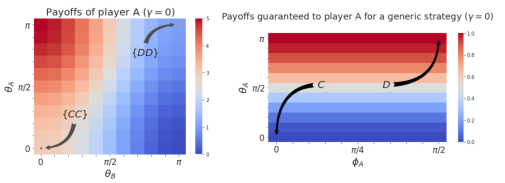
\includegraphics[width=0.5\textwidth]{pictures/utilities_gamma0.pdf}
	\caption{Utilities of the contender A in a game with $\gamma=0$, as function of the strategies chosen (left). Minimum payoff guaranteed to A for a generic strategy of B (right).}
	\label{fig:utilA_gamma0}
\end{figure}

The situation is entirely different for a maximally entangled game, with $\gamma=\pi/2$: this time, any pair of strategies chosen will have no counterpart in the classical domain, providing new and interesting solutions. To be precise, one can always re-derive the original prisoners' dilemma if both players choose actions of the type $\hat{U}(\pi/2,0)$. From the numerical analysis of the problem \cite{Pujatti_github}, one can clearly observe that there are no dominant strategies this time, and this means that $\{\hat{D}\hat{D}\}$ is no longer an equilibrium in dominant strategies. Furthermore, such NE is replaced by a new joint strategy of best replies (from which no rational player would deviate), i.e. $\{\hat{Q}\hat{Q}\}$. 
\[ \hat{Q} \equiv \hat{U}(0,\frac{\pi}{2}) = \begin{pmatrix} i&0\\0&-i \end{pmatrix} \]
This is the new unique equilibrium of the game, and guarantees a final payoff of 3 for both players; in fact
\[ payoff_A(\hat{Q},\hat{U}_B)=\cos^2\left(\frac{\theta}{2}\right)\left(3\sin^2\phi + \cos^2\phi \right)\leq 3 \quad \forall\theta,\phi \]
and the same holds for Bob.\\
Using the same representation as before, according to the payoff plot \ref{fig:utilBvsQ} of player B, notice that, assuming that the first player chooses this new optimal strategy $\hat{Q}$, then there is no choice for the second that would improve his payoff rather than $\hat{Q}$ as well.\\ 

\begin{figure}[!ht]
	\centering
	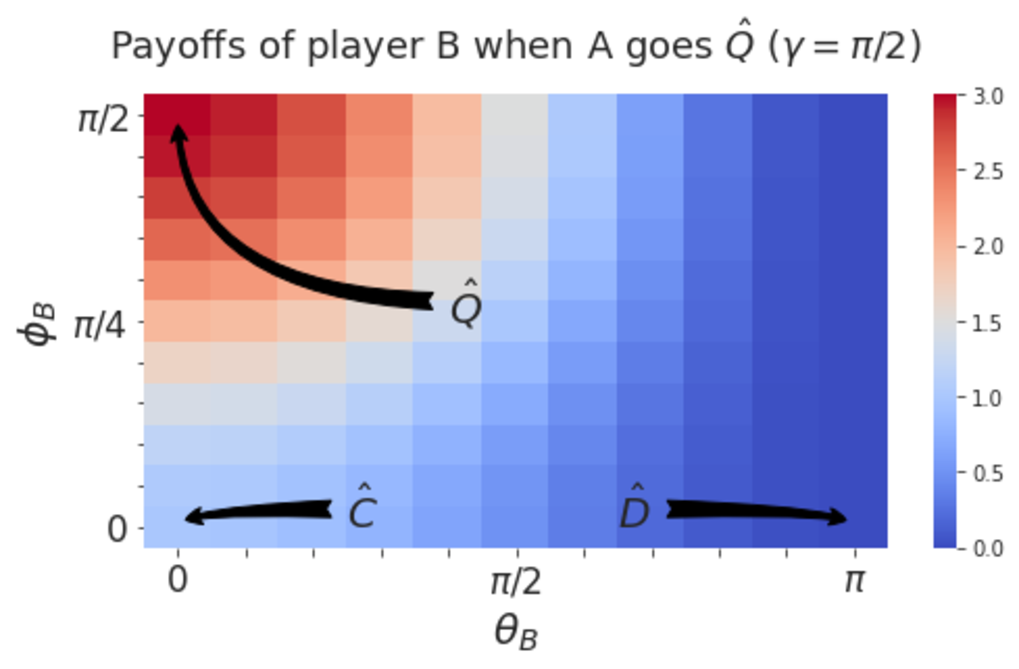
\includegraphics[scale=0.5]{pictures/payoffsBvsQ.pdf}
	\caption{Utilities of player B when A selects the optimal strategy $\hat{Q}$.}
	\label{fig:utilBvsQ}
\end{figure}

Moreover, $\hat{Q}\otimes\hat{Q}$ is not just a Nash equilibrium but has also the property of being \textit{Pareto Optimal}, meaning that deviating from this pair of strategies it is not possible to increase the payoff of one player
without reducing the utility of the other. The solution of the classical game was not Pareto optimal: the only strategy with this property was the mutual cooperation, but such choice was not holdable by rational players without considering a multistage game (with carrot and stick or grim trigger approaches). And this is the first advantage provided by the quantum transposition of the game since, in a certain sense, the dilemma has just been solved.\\

\subsection{Quantum player vs Classical opponent}
What if the game was instead unfair like the spin-flip example presented in the second section, in the sense that quantum strategies are accessible only to one player?\\
Suppose that Alice has studied quantum mechanics, so her state space is still $SU(2)$, while Bob is limited to select actions characterized by $\phi=0$: in this case A is well advised to play the so called \textit{miracle move} (according to Eisert et al. \cite{Eisert_2020})
\[ \hat{M}\equiv\hat{U}(\pi/2,\pi/2)=\frac{1}{\sqrt{2}}\begin{pmatrix} i&-1\\1&-i \end{pmatrix}  \]
that guarantees the following payoffs
\[ payoff_A\left(\hat{M},\hat{U}(\theta,0)\right) \geq 3 \quad payoff_B\left(\hat{M},\hat{U}(\theta,0)\right) \leq \frac{1}{2}  \]
The comparison among the possible combinations of actions is shown in figure \ref{fig:quantumvsclassical}.\\

\begin{figure}[!ht]
	\centering
	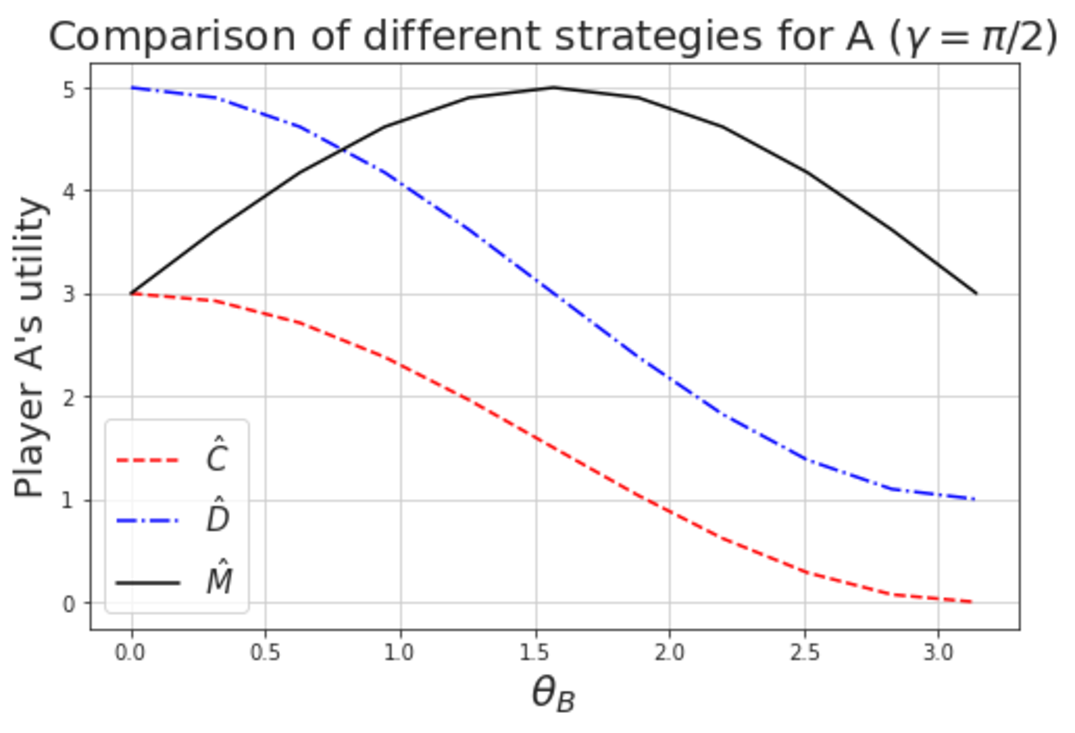
\includegraphics[scale=0.4]{pictures/PD_quantumvsclassical.pdf}
	\caption{Final payoffs for different strategies selected by Alice, as function of the parameter $\theta_B$.}
	\label{fig:quantumvsclassical}
\end{figure}

So player A (rationally) will play "always $\hat{M}$", since this strategy will give her a utility of at least 3, regardless of the strategy chosen by B, which is inevitably in a position of disadvantage. This approach certainly outperforms "tit-for-tat", at least in these kind of asymmetric problems.\\
Finally, it may be interesting to study also the effective payoff of the quantum player as a function of the degrees of entanglement of the game, i.e. the parameter $\gamma$. The minimal expected payoff accessible by Alice is given by
\[ m = \max_{\hat{U}_A\in SU(2)}\min_{\hat{U}_B\in\{\hat{C},\hat{D}\}} payoff_A\left(\hat{U}_A, \hat{U}_B\right) \]
and the plot realized is shown in figure \ref{fig:payoffs_entanglement_PD}. 

\begin{figure}[!ht]
	\centering
	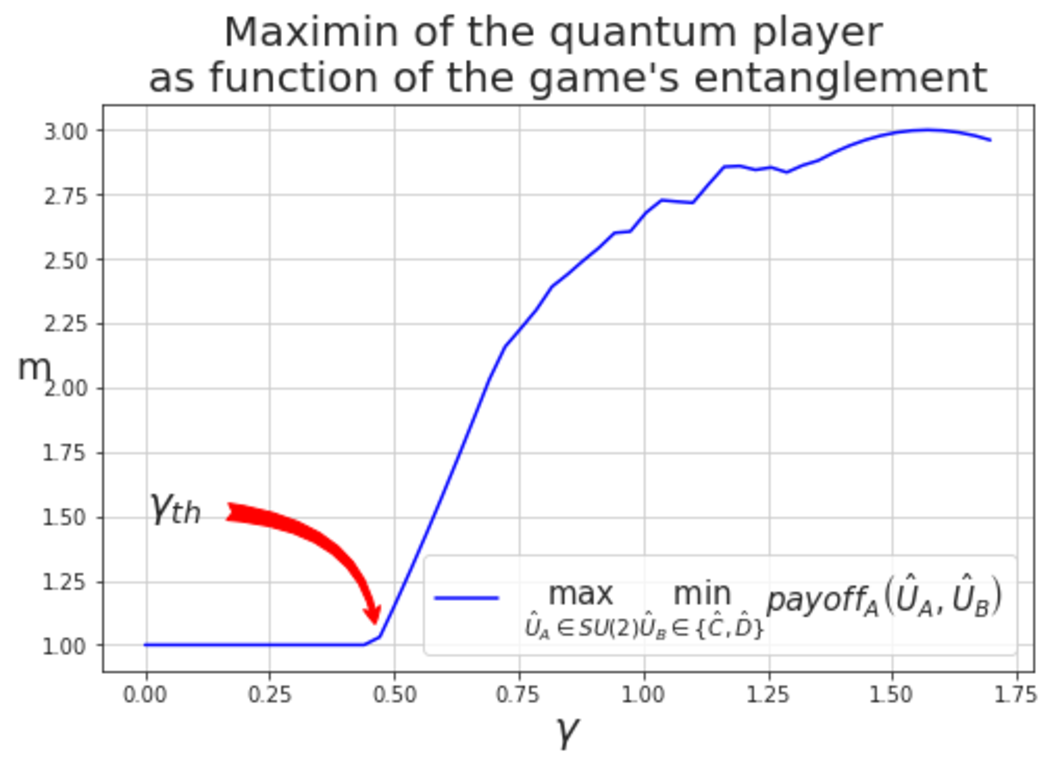
\includegraphics[scale=0.45]{pictures/PD_payoffsentanglement.pdf}
	\caption{Payoffs guaranteed to player A as function of the entanglement measure $\gamma$.}
	\label{fig:payoffs_entanglement_PD}
\end{figure}


It is immediately possible to notice that under a certain threshold, in term of entanglement degrees, that is found to be around $\gamma_{th} = \arcsin\left(1/\sqrt{5}\right)\simeq 0.464$, the forced choice is playing $\hat{F}$; after such threshold, near to the maximum entanglement among the states, then the best reply is always the miracle move. An interesting fact, not shown by the graph because of the limited precision, is that the "strategy swap", from $\hat{F}$ to $\hat{Q}$ is much more discontinuous than how it appears: this is a clue that a phenomenon known as \textit{quantum phase transition} has occurs around $\gamma_{th}$.	




